\section{Evaluation} %%%%%%%%%%%%%%%%%%%%%%%%%%%%%%%%%%%%%%%%%%%%%%%%%%%%%%%%%%%
\label{sec:eval}

\begin{figure*}
\begin{tabular}{@{}c@{ }l||@{ }r@{}@{ }r@{}|@{ }r@{}@{ }r@{}||@{ }r@{}@{ }r@{}|@{ }r@{}@{ }r@{}||@{ }r@{}@{ }r@{}|@{ }r@{}@{ }r@{}||@{ }r@{}@{ }r@{}|@{ }r@{}@{ }r@{}}
\hline % -----------------------------------------------------------------------------------------------------------------------------------------
\hline % -----------------------------------------------------------------------------------------------------------------------------------------
 &            & \multicolumn{4}{c||}{G++/32}  & \multicolumn{4}{c||}{G++/32}  & \multicolumn{4}{c||}{MS Visual C++/32} & \multicolumn{4}{c}{MS Visual C++/64} \\
\hline % -------------------------------------------------------------------------------------------------------------------------------------------------------------------------
 & Syntax     & \multicolumn{2}{c|}{Unified} & \multicolumn{2}{c||}{Special} & \multicolumn{2}{c|}{Unified} & \multicolumn{2}{c||}{Special} & \multicolumn{2}{c|}{Unified} & \multicolumn{2}{c||}{Special} & \multicolumn{2}{c|}{Unified} & \multicolumn{2}{c}{Special} \\
\hline % -------------------------------------------------------------------------------------------------------------------------------------------------------------------------
 & Encoding   & \Opn  & \Cls  & \Opn  & \Cls  & \Opn  & \Cls  & \Opn  & \Cls  & \Opn  & \Cls  & \Opn  & \Cls  & \Opn  & \Cls  & \Opn  & \Cls   \\
\hline % ----------------------------------------------------------------------------------------------------------------------------------
\hline % ----------------------------------------------------------------------------------------------------------------------------------
 & Repetitive &\glNGPp&\glNGKp&\glNSPp&\glNSKp&\gwNGPp&\gwNGKp&\gwNSPp&\gwNSKp&\VwNGPp&\VwNGKp&\VwNSPp&\VwNSKp&\VxNGPp&\VxNGKp&\VxNSPp&\VxNSKp \\
 & Sequential &\glNGPq&\glNGKq&\glNSPq&\glNSKq&\gwNGPq&\gwNGKq&\gwNSPq&\gwNSKq&\VwNGPq&\VwNGKq&\VwNSPq&\VwNSKq&\VxNGPq&\VxNGKq&\VxNSPq&\VxNSKq \\
 & Random     &\glNGPn&\glNGKn&\glNSPn&\glNSKn&\gwNGPn&\gwNGKn&\gwNSPn&\gwNSKn&\VwNGPn&\VwNGKn&\VwNSPn&\VwNSKn&\VxNGPn&\VxNGKn&\VxNSPn&\VxNSKn \\
\hline % ----------------------------------------------------------------------------------------------------------------------------------
\multirow{3}{*}{\begin{sideways}{\tiny Forward}\end{sideways}}
 & Repetitive &\glYGPp&\glYGKp&\glYSPp&\glYSKp&\gwYGPp&\gwYGKp&\gwYSPp&\gwYSKp&\VwYGPp&\VwYGKp&\VwYSPp&\VwYSKp&\VxYGPp&\VxYGKp&\VxYSPp&\VxYSKp \\
 & Sequential &\glYGPq&\glYGKq&\glYSPq&\glYSKq&\gwYGPq&\gwYGKq&\gwYSPq&\gwYSKq&\VwYGPq&\VwYGKq&\VwYSPq&\VwYSKq&\VxYGPq&\VxYGKq&\VxYSPq&\VxYSKq \\
 & Random     &\glYGPn&\glYGKn&\glYSPn&\glYSKn&\gwYGPn&\gwYGKn&\gwYSPn&\gwYSKn&\VwYGPn&\VwYGKn&\VwYSPn&\VwYSKn&\VxYGPn&\VxYGKn&\VxYSPn&\VxYSKn \\
\hline % ----------------------------------------------------------------------------------------------------------------------------------
\hline % ----------------------------------------------------------------------------------------------------------------------------------
 &            & \multicolumn{4}{c||}{Linux Desktop} & \multicolumn{12}{c}{Windows 7 Laptop}                                                    \\
\hline % ----------------------------------------------------------------------------------------------------------------------------------
\end{tabular}
\caption{Relative performance of our pattern matching versus visitors. Numbers 
in bold font (e.g. \f{67}), indicate that our pattern matching is faster than 
visitors by corresponding percentage. Numbers in italics font (e.g. \s{14}), 
indicate that our solution is slower than visitors (i.e. visitors is faster than 
our solution) by corresponding percentage.}
\label{relperf}
\end{figure*}

Our evaluation methodology consists of several benchmarks that represent various 
uses of objects inspected with either visitors or type switching.

The \emph{repetitive} benchmark performs multiple calls on different objects of the 
same most derived type. This scenario happens in object-oriented setting when a 
group of polymorphic objects is created and passed around (e.g. numerous 
particles of a given kind in a particle simulation system). We include it 
because double dispatch becomes about twice faster (27 vs. 53 cycles) in this 
scenario compared to others due to cache and call target prediction mechanisms. 

The \emph{sequential} benchmark effectively uses an object of each derived type only 
once and then moves on to an object of a different type. The cache is typically 
reused the least in this scenario, which is typical of lookup tables, where each 
entry is implemented with a different derived class.

The \emph{random} benchmark is the most representative as it randomly makes calls on 
random objects, which will probably be the most common usage scenario in the 
real world.

The \emph{forwarding} benchmark is not a benchmark on its own, but rather a 
combinator that can be applied to any of the above scenarios. It refers to the 
common technique used by visitors where, for class hierarchies with multiple 
levels of inheritance, the \code{visit} method of a derived class will provide a 
default implementation of forwarding to its immediate base class, which, in turn, 
may forward it to its base class, etc. The use of forwarding in visitors is a 
way to achieve substitutability, which in type switches corresponds to the use 
of base classes in the case clauses.

The class hierarchy for non-forwarding test was a flat hierarchy with 100 
derived classes, encoding an algebraic data type. The class hierarchy for 
forwarding tests had two levels of inheritance with 5 intermediate base classes 
and 95 derived ones. 

Each benchmark was tested with either \emph{unified} or \emph{specialized} 
syntax, each of which included tests on polymorphic (\emph{Open}) and tagged 
(\emph{Tag}) encodings. Specialized syntax avoids generating unnecessary 
syntactic structure used to unify syntax, and thus produces faster code. We 
include it in our results because a compiler implementation of type switching 
will only generate the best suitable code.

The benchmarks were executed in the following configurations:

\begin{itemize}
\setlength{\itemsep}{0pt}
\setlength{\parskip}{0pt}
\item Dell Dimension\textsuperscript{\textregistered} desktop with Intel\textsuperscript{\textregistered} Pentium\textsuperscript{\textregistered} 
      D (Dual Core) CPU at 2.80 GHz; 1GB of RAM; Fedora Core 13  
      \begin{itemize}
      \setlength{\itemsep}{0pt}
      \setlength{\parskip}{0pt}
      \item G++ 4.4.5 executed with -O2
      \end{itemize}
\item Sony VAIO\textsuperscript{\textregistered} laptop with Intel\textsuperscript{\textregistered} Core\texttrademark i5 460M 
      CPU at 2.53 GHz; 6GB of RAM; Windows 7 Professional
      \begin{itemize}
      \setlength{\itemsep}{0pt}
      \setlength{\parskip}{0pt}
      \item G++ 4.5.2 / MinGW executed with -O2; x86 binaries
      \item MS Visual C++ 2010 Professional x86/x64 binaries with Profile-Guided Optimizations
      \end{itemize}
\end{itemize}

The code on the critical path of our type switch implementation benefits 
significantly from branch hinting as some branches are much more likely than 
others. We use the branch hinting in GCC to guide the compiler, but, 
unfortunately, Visual C++ does not have similar facilities. Microsoft suggests 
to use \emph{Profile-Guided Optimization} to achieve the same, which is why the 
results for Visual C++ reported here have been obtained with profile-guided 
optimizations enabled. The results without profile-guided optimizations can be 
found in the accompanying technical report~\cite{TR}.
%The results of optimizing code created with Visual C++ by using profile 
%guided optimizations as currently Visual C++ does not have means for branch 
%hinting, which are supported by G++ and proven to be very effective in few 
%cruicial places. Profile guided optimization in Visual C++ lets compiler find 
%out experimentally what we would have otherwise hinted, even though this 
%includes other optimizations as well.

We compare the performance of our solution relative to the performance of visitors in 
Figure~\ref{relperf}. The values are given as percentages of performance increase 
against the slower technique. Numbers in bold represent cases where our type 
switching was faster than visitors were. Numbers in italics indicate cases where 
visitors were faster.

We can see that type switching wins by a good margin in the presence of at least 
one level of forwarding on visitors. Using type switching on closed hierarchies 
is also a definite winner. Note that the numbers are relative, and thus the 
ratio depends on both the performance of virtual calls and the performance of 
switch statements. Visual C++ was generating faster virtual function calls, 
while GCC was generating faster switch statements, which is why their relative 
performance seem to be much more favorable for us in the case of GCC.

Similarly the code for x64 is only slower relatively: the actual time spent for 
both visitors and type switching was smaller than that for x86, but it was much 
smaller for visitors than type switching, which resulted in worse relative 
performance.

\subsection{V-Table Pointer Memoization vs. Tag Precedence List}
\label{sec:cmp}

With a few exceptions for x64, it can be seen from Figure~\ref{relperf} 
that the performance of the tag precedence list approach (the Tag column) dominates the 
performance of the v-table pointer memoization approach (the Open column). We believe 
that the difference, often significant, is the price one pays for the true 
openness of the v-table pointer memoization solution.

Unfortunately, the tag precedence list approach is not truly open. The use of tags, 
even if they would be allocated by compiler, may require integration efforts to 
ensure that different DLLs have not reused the same tags. Randomization of tags,
similar to a proposal of Garrigue~\cite{garrigue-98}, will not eliminate the 
problem and will surely replace jump tables in switches with decision trees. This 
will likely significantly degrade the numbers for the Tag column of 
Figure~\ref{relperf}, since the tags in our experiments were all sequential.

Besides, the tag precedence list approach relies on static cast to obtain the 
proper reference once the most specific case clause has been found. As we 
described in \textsection\ref{sec:vtblmem}, this has severe limitations in the 
presence of multiple inheritance, and thus is not as versatile as the other 
solution. Overcoming this problem will either require the use of 
\code{dynamic_cast} or techniques similar to those we used in v-table pointer 
memoization. This will likely degrade performance numbers for the Tag column even further.

Note also that the v-table pointer memoization approach can be used to implement both
first-fit and best-fit semantics, while the tag precedence list is only suitable 
for best-fit semantics. Their complexity guarantees also differ: v-table pointer 
memoization is constant on average, and slow on the first call. Tag list approach is 
logarithmic in the size of the class hierarchy on average (assuming a balanced 
hierarchy), including on the first call.

\subsection{Comparison with OCaml}
\label{sec:ocaml}

We now compare our solution to the built-in pattern-matching facility of OCaml. 
In this test, we timed a small OCaml application performing our sequential 
benchmark on an algebraic data type of 100 variants. Corresponding C++ 
applications were working with a flat class hierarchy of 100 derived classes. 
The difference between the C++ applications lies in the encoding (Open/Tag/Kind) 
and the syntax (Uni/Spec) used. Kind encoding is the same as Tag encoding, but 
it does not require substitutability, and thus can be implemented with a direct 
switch on tags. It is only supported through specialized syntax in our library 
as it differs from the Tag encoding only semantically.

The optimized OCaml compiler \texttt{ocamlopt.opt} that we used to compile the code 
can be based on different toolkits on some platforms, e.g. Visual C++ or GCC 
under Windows. To make the comparison fair we thus had to make sure that the 
same toolkit was used to compile the corresponding C++ code. We ran the tests 
on both of the machines described above using the following configurations: 

\begin{itemize}
\setlength{\itemsep}{0pt}
\setlength{\parskip}{0pt}
\item The tests on a Windows 7 laptop were all based on the \emph{Visual C++ toolset} 
      and used \texttt{ocamlopt.opt} version 3.11.0.
\item The tests on a Linux desktop were all based on the \emph{GCC toolset} and used 
      \texttt{ocamlopt.opt} version 3.11.2
\end{itemize}

The timing results presented in Figure~\ref{fig:OCamlComparison} are averaged 
over 101 measurements and show the number of seconds it took to perform a 
million decompositions within our sequential benchmark.

\begin{figure}[htbp]
  \centering
    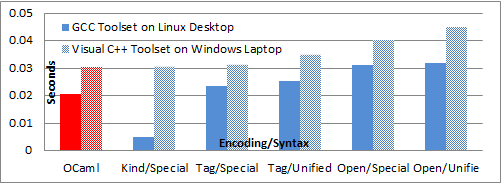
\includegraphics[width=0.47\textwidth]{OCamlComparison.png}
  \caption{Performance comparison of various encodings and syntax against OCaml code}
  \label{fig:OCamlComparison}
\end{figure}

We can see that the use of specialized syntax on a closed/sealed hierarchy can 
match the speed of, and even be four times faster than, the code generated by 
the native OCaml compiler. Once we go for an open solution, we become about 
30-50\% slower. 
